\begin{figure}[!ht]
\centering
\subfloat[Diffuse color]{\resizebox{50mm}{!}{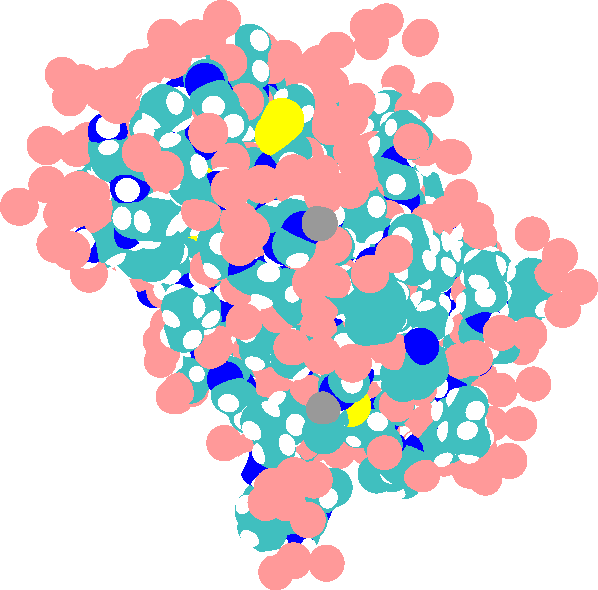
\includegraphics{img/albedo.png}}}
\subfloat[Eye-space normals]{\resizebox{50mm}{!}{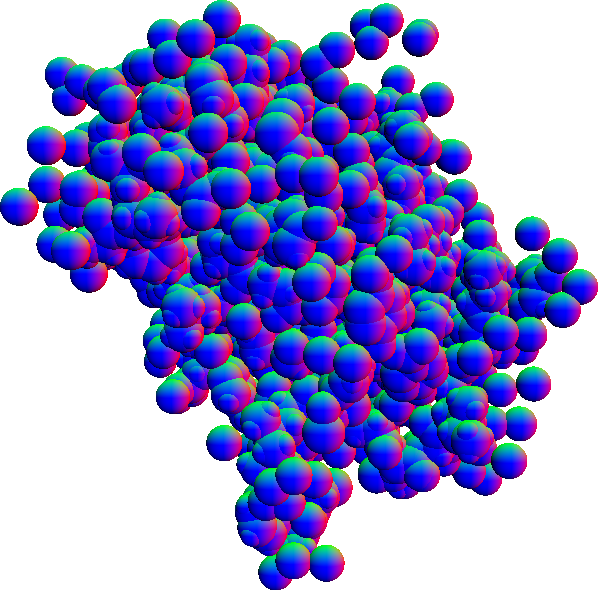
\includegraphics{img/normals.png}}}
\subfloat[Approximation of depth ($\mu$)]{\resizebox{50mm}{!}{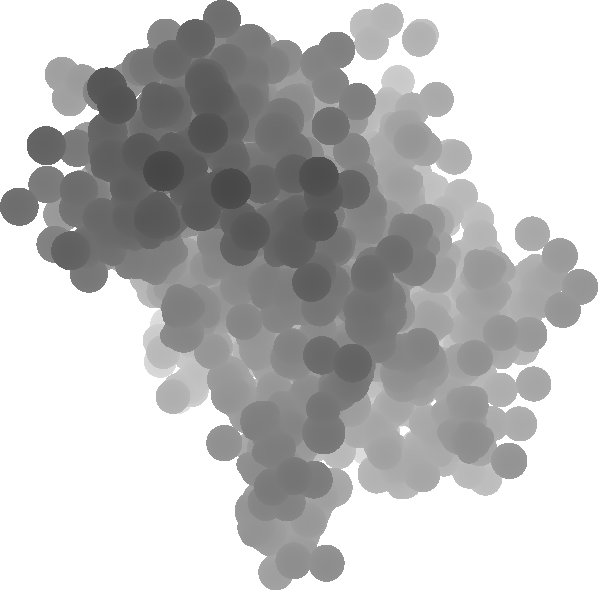
\includegraphics{img/depth.png}}}

\subfloat[Phong shading]{\resizebox{50mm}{!}{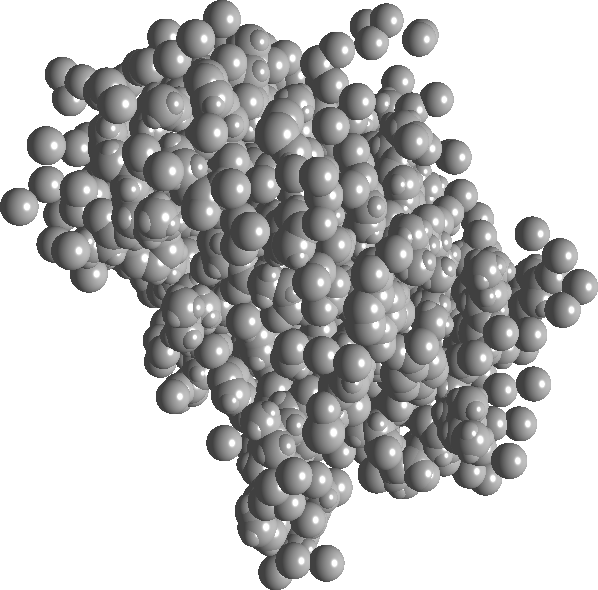
\includegraphics{img/shading.png}}}
\subfloat[Silhouette outlines]{\resizebox{50mm}{!}{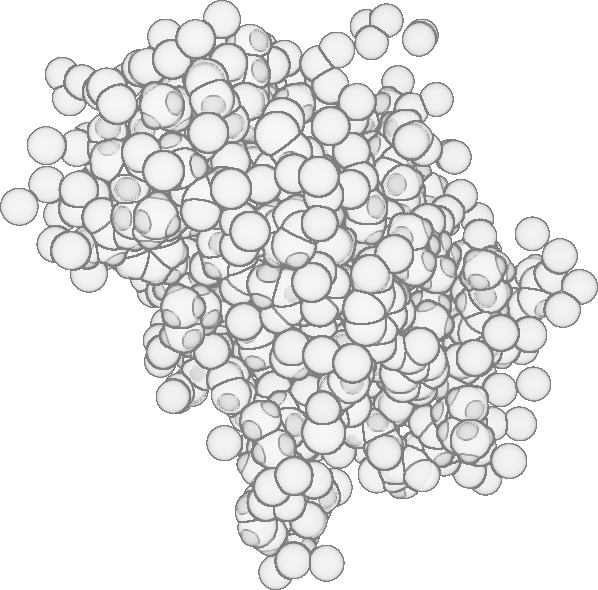
\includegraphics{img/silhouette.png}}}
\subfloat[Final composite image]{\resizebox{50mm}{!}{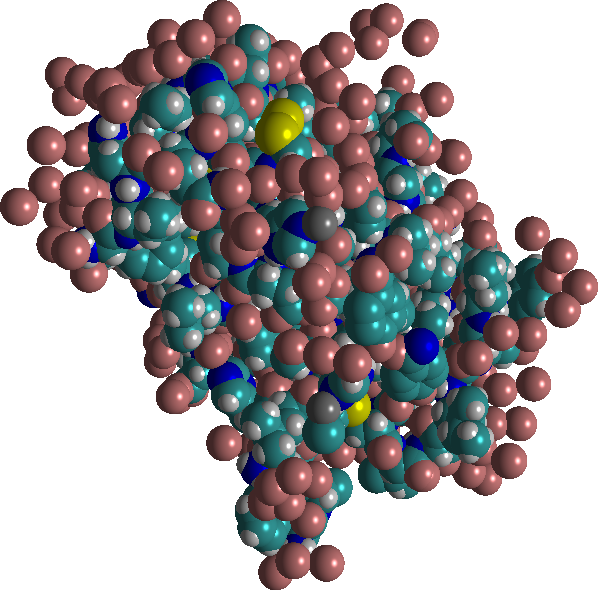
\includegraphics{img/final.png}}}
\caption{\em Buffers and effects generated during rendering of a deferred shaded image with silhouette outlines}
\label{f:steps}
\end{figure}

\section{Results}

The quality of the images rendered by our custom quadric ray-caster closely match those of Sigg's paper (Fig. \ref{f:steps}).
On first impression, the performance is very good; on a mid-range GeForce 8600 GT is fluid enough in most cases to be considered real-time.

\subsection*{Performance}
Since Sigg uses a different testing system, and our implementation differs in several ways (i.e. no shadow maps, differences in efficiency, different
scene setup), our performance numbers can not be directly compared. However, we might be able to see similar patterns in the figures.

All benchmarks are performed at a resolution of 1024$\times$768. 
Our default testing system is an Intel Core 2 Duo E6550 (2.33 GHz) with 2 GB RAM and a GeForce 8600 GT graphics card.

The data sets used for the tests are the same as those used by Sigg. 
Some sets represent the same molecule structures, but with different sized spheres.
A list of all these data sets, along with the abbreviations used in this section, is available in Appendix \ref{app:labels}.

Our benchmarking method is as follows. 
The camera is positioned at one of three different distances from the model. 
The model rotates at a constant speed, while the rendered frames are counted.
After ten seconds, the benchmarks stops and the average number of frames per second is reported.

Cylinders are not taken along in the benchmarks, because they are not properly optimized and would therefore skew the results.

\subsubsection*{Sphere count}

First, we see how the number of spheres in a model affects the performance. 
This benchmark was run on the default system, with the camera at 5 units distance from the center of each data set.
The three different shading types (direct shading, normal deferred shading, deferred shading with silhouette lines) have all been tested.
The results of the benchmarks are shown in Figure \ref{f:spherecount}.

\begin{figure}[!ht]
\centering
\resizebox{120mm}{!}{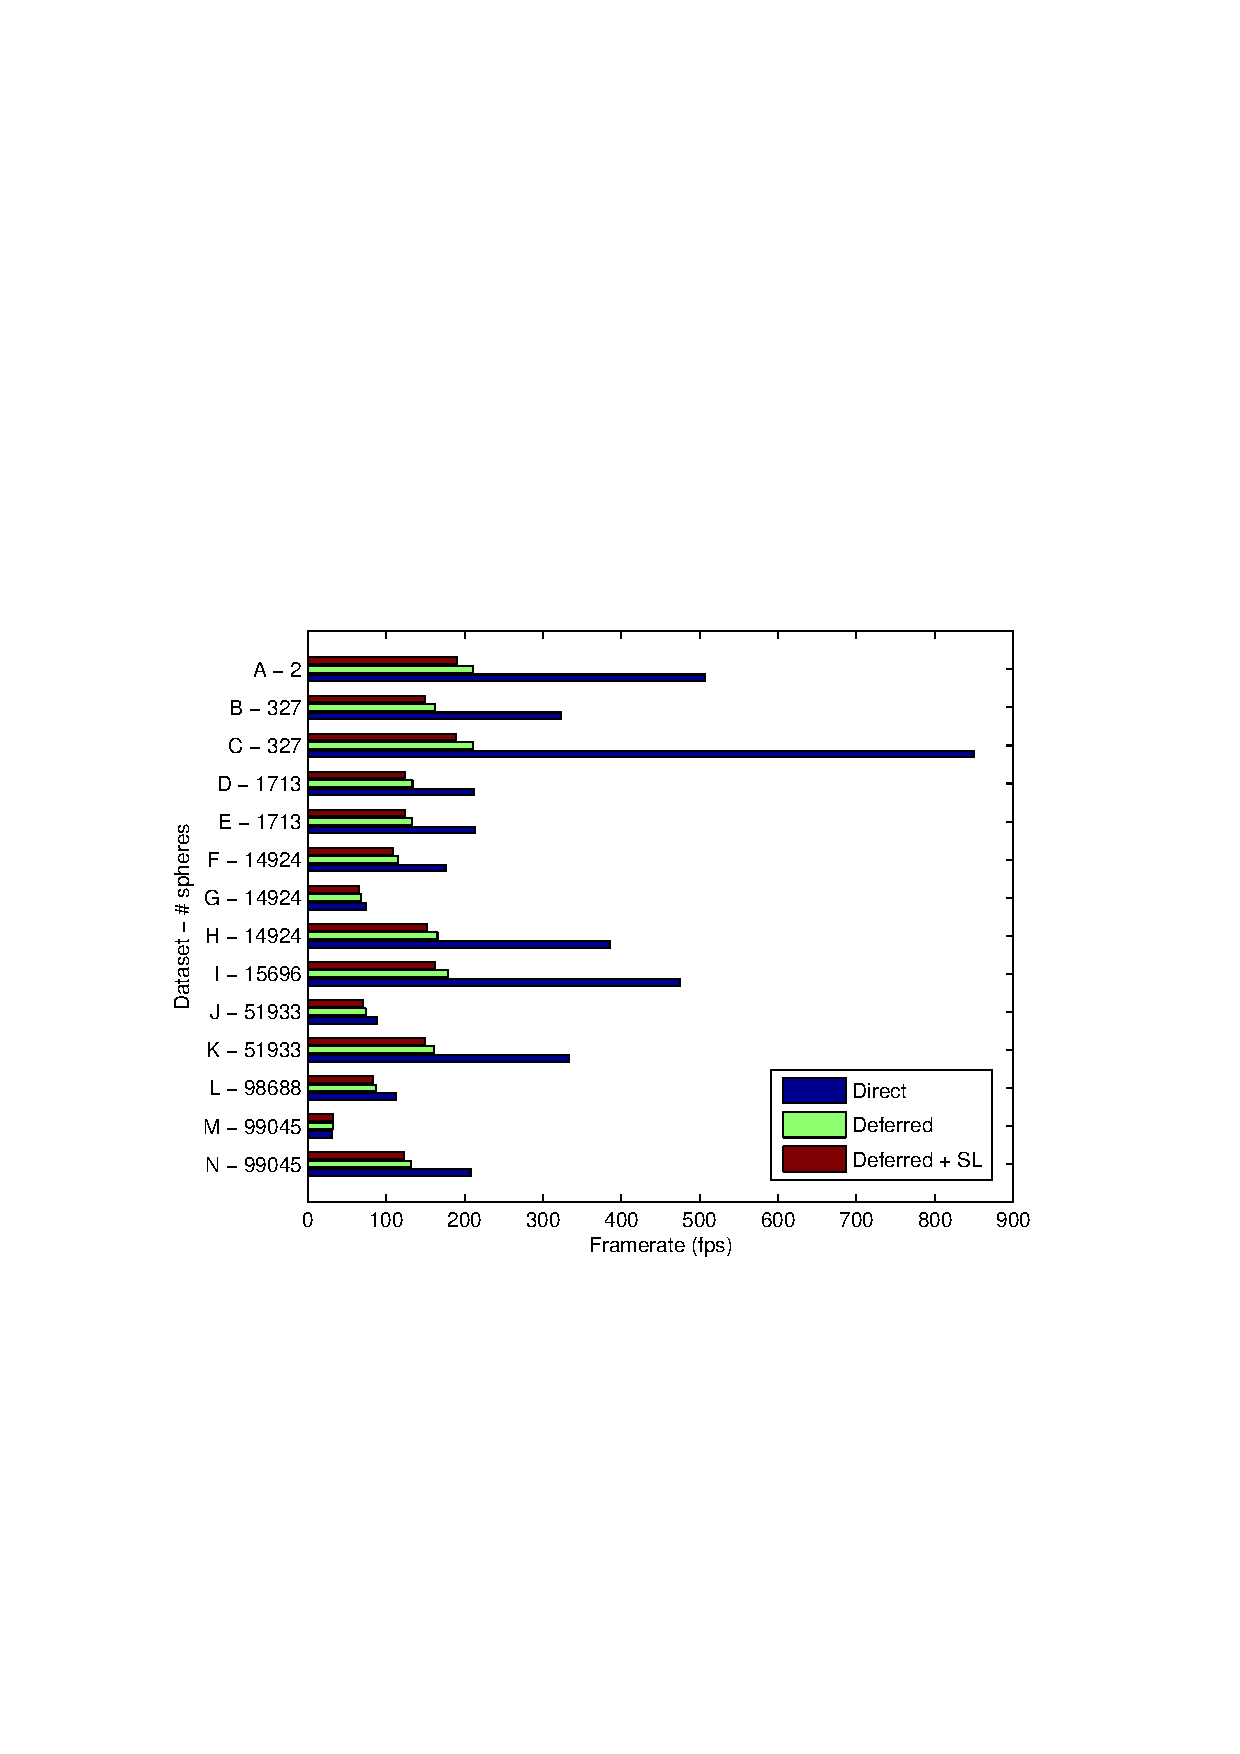
\includegraphics{img/dataset_vs_fps_8600gt_cam5.pdf}}
\caption{\em Performance impact from the number of spheres}
\label{f:spherecount}
\end{figure}

Although a larger number of spheres generally does decrease the performance, 
there are also cases where a small number of spheres has worse performance than a larger number of spheres (e.g. data set G vs. data set K).
It seems there are factors other than the raw number of spheres that strongly affect the performance.
This was also notable in Sigg's performance results.

What's also directly visible is that deferred shading is generally slower than direct shading.
Apparantly, the memory bandwidth requirements for deferred shading outweigh the lower number of shading calculations that it yields.
In Sigg's paper, deferred shading was only faster than direct shading when shadow mapping was applied.
This is something we can not test with our implementation, but we might be able to create a situation where the balance between 
shader performance and memory bandwidth shifts.

\subsubsection*{Camera distance}

During basic testing, it became clear that the proximity of the spheres to the camera was crucial in the performance of the renderer.
This is visible in the screenshots from Figure \ref{f:camdist}.

\begin{figure}[!ht]
\centering
\subfloat[Distance = 5, fps = 20.6]{\resizebox{50mm}{!}{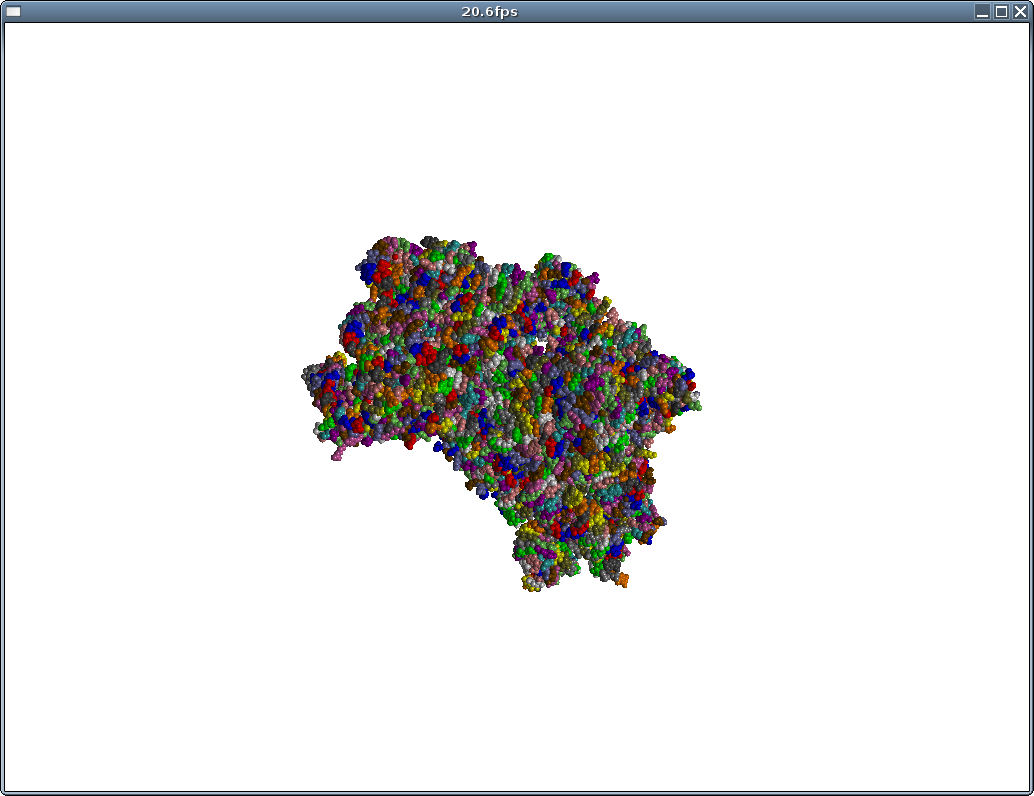
\includegraphics{img/cam5.png}}}
\subfloat[Distance = 3, fps = 13.3]{\resizebox{50mm}{!}{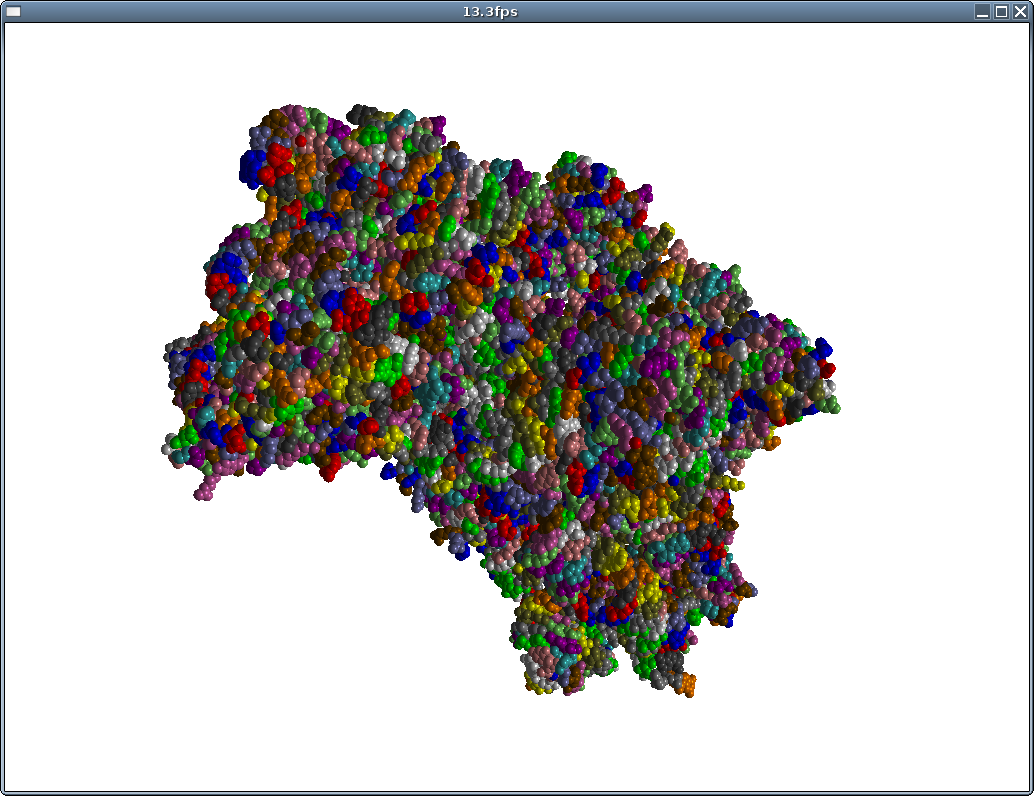
\includegraphics{img/cam3.png}}}
\subfloat[Distance = 1, fps = 4.1]{\resizebox{50mm}{!}{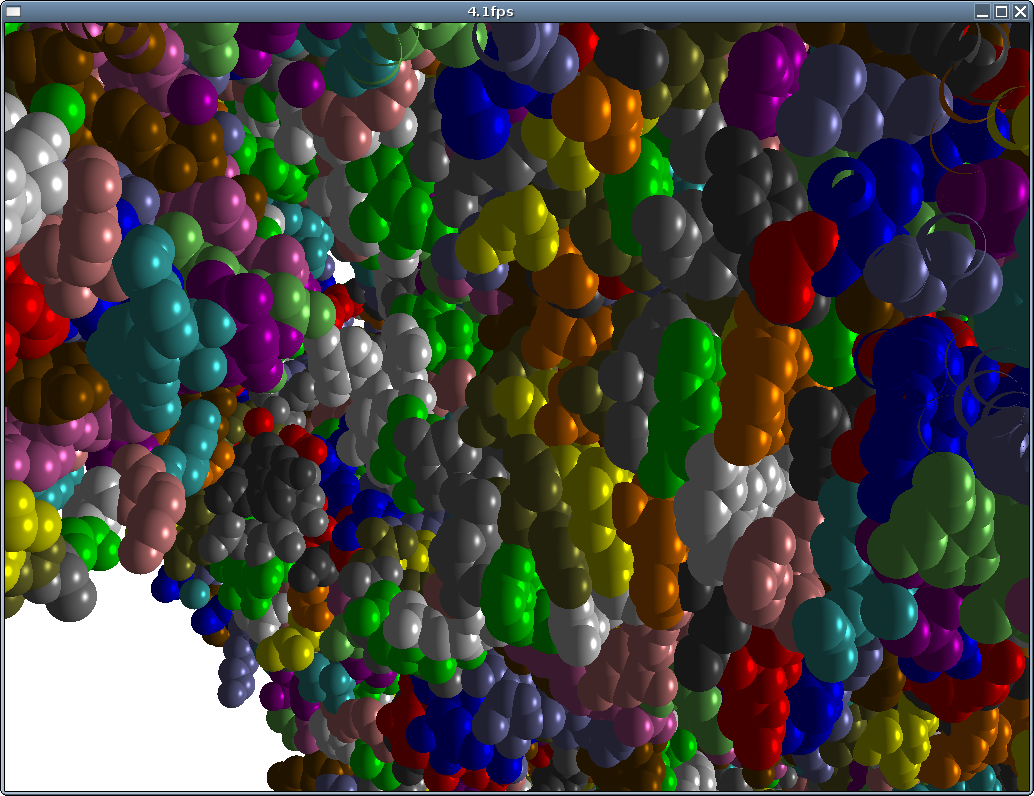
\includegraphics{img/cam1.png}}}
\caption{\em Camera position affecting performance on a GeForce 8400 GS}
\label{f:camdist}
\end{figure}

To verify this observation, we have performed several tests on two dense sets of spheres, with varying camera distances.
The results of these tests are shown in Figure \ref{f:cam-dist}.

\begin{figure}[!ht]
\centering
\subfloat[Dataset M]{\resizebox{75mm}{!}{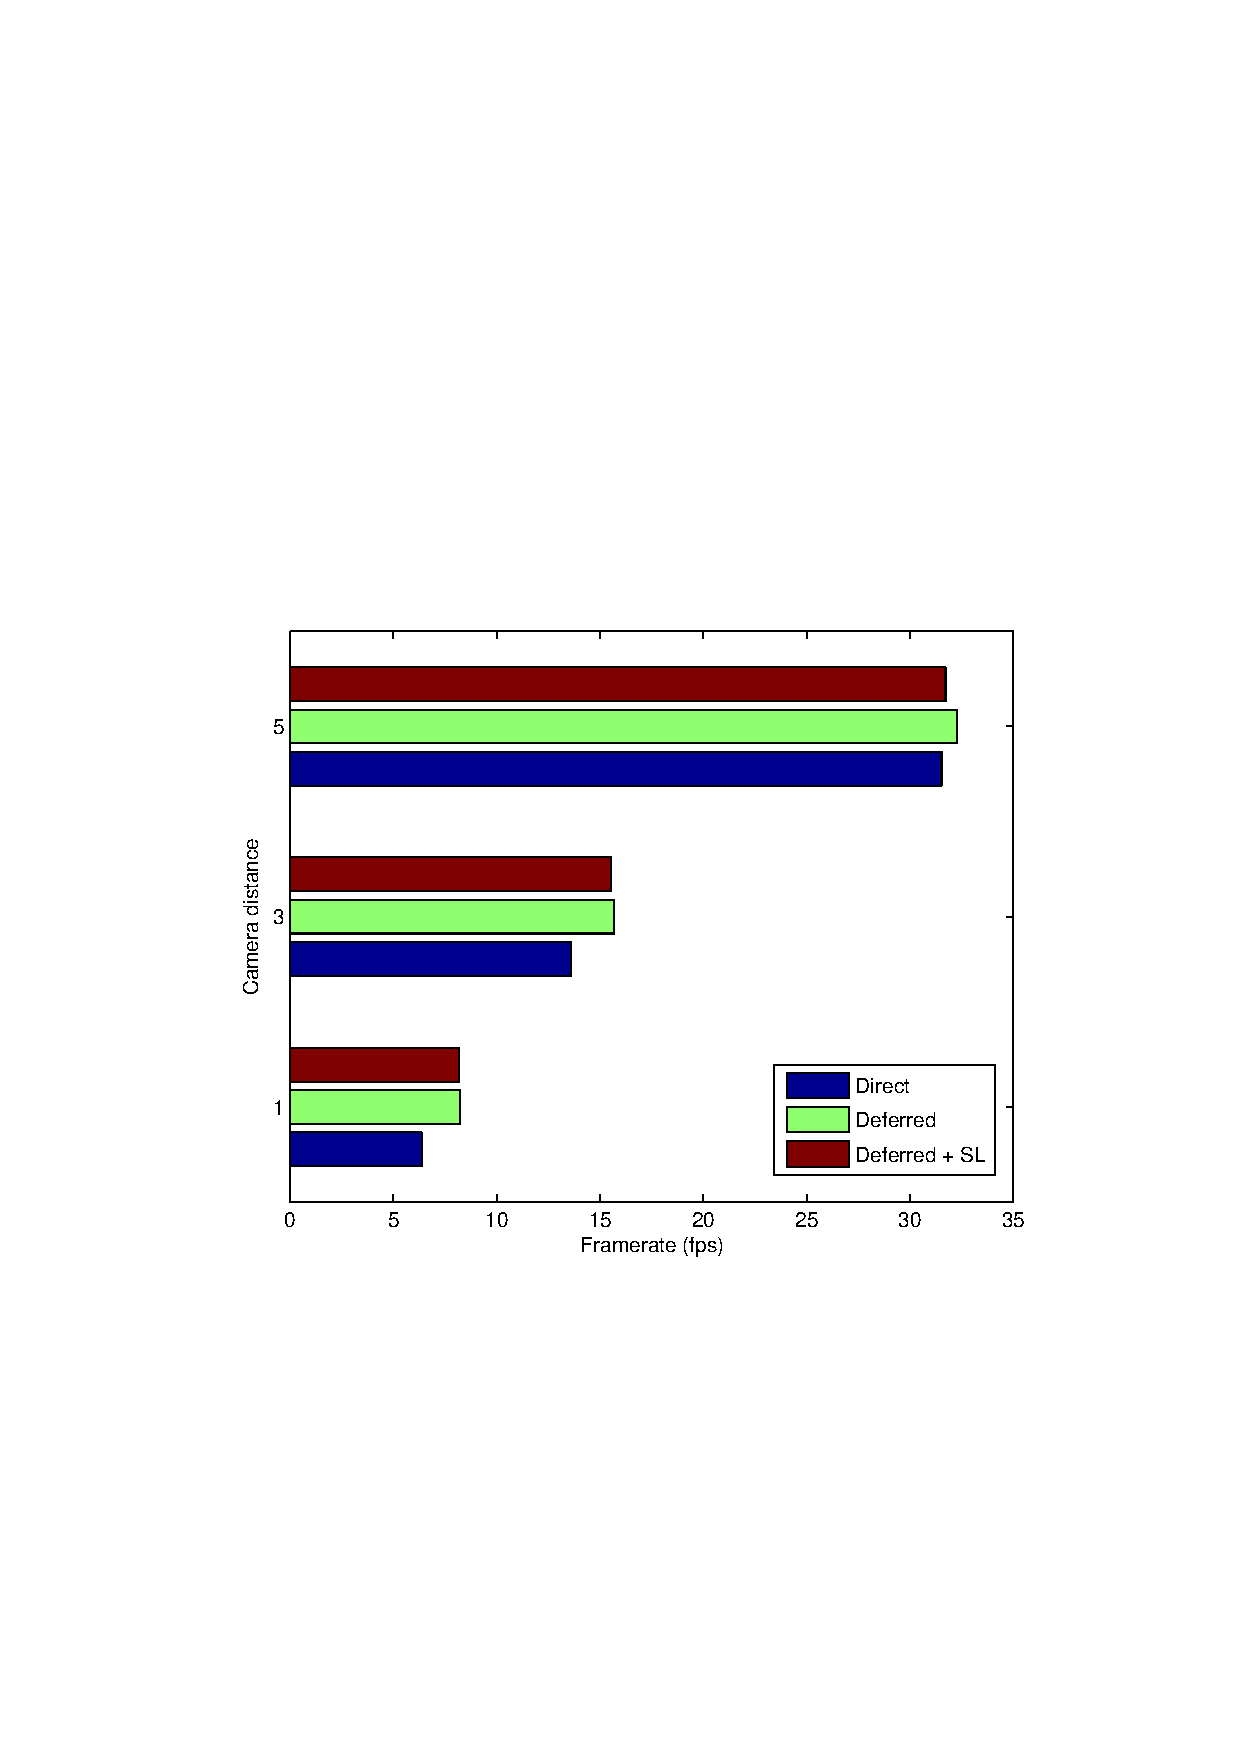
\includegraphics{img/camdist_vs_fps_8600gt_1vqm-vdw.pdf}}}
\subfloat[Dataset N]{\resizebox{75mm}{!}{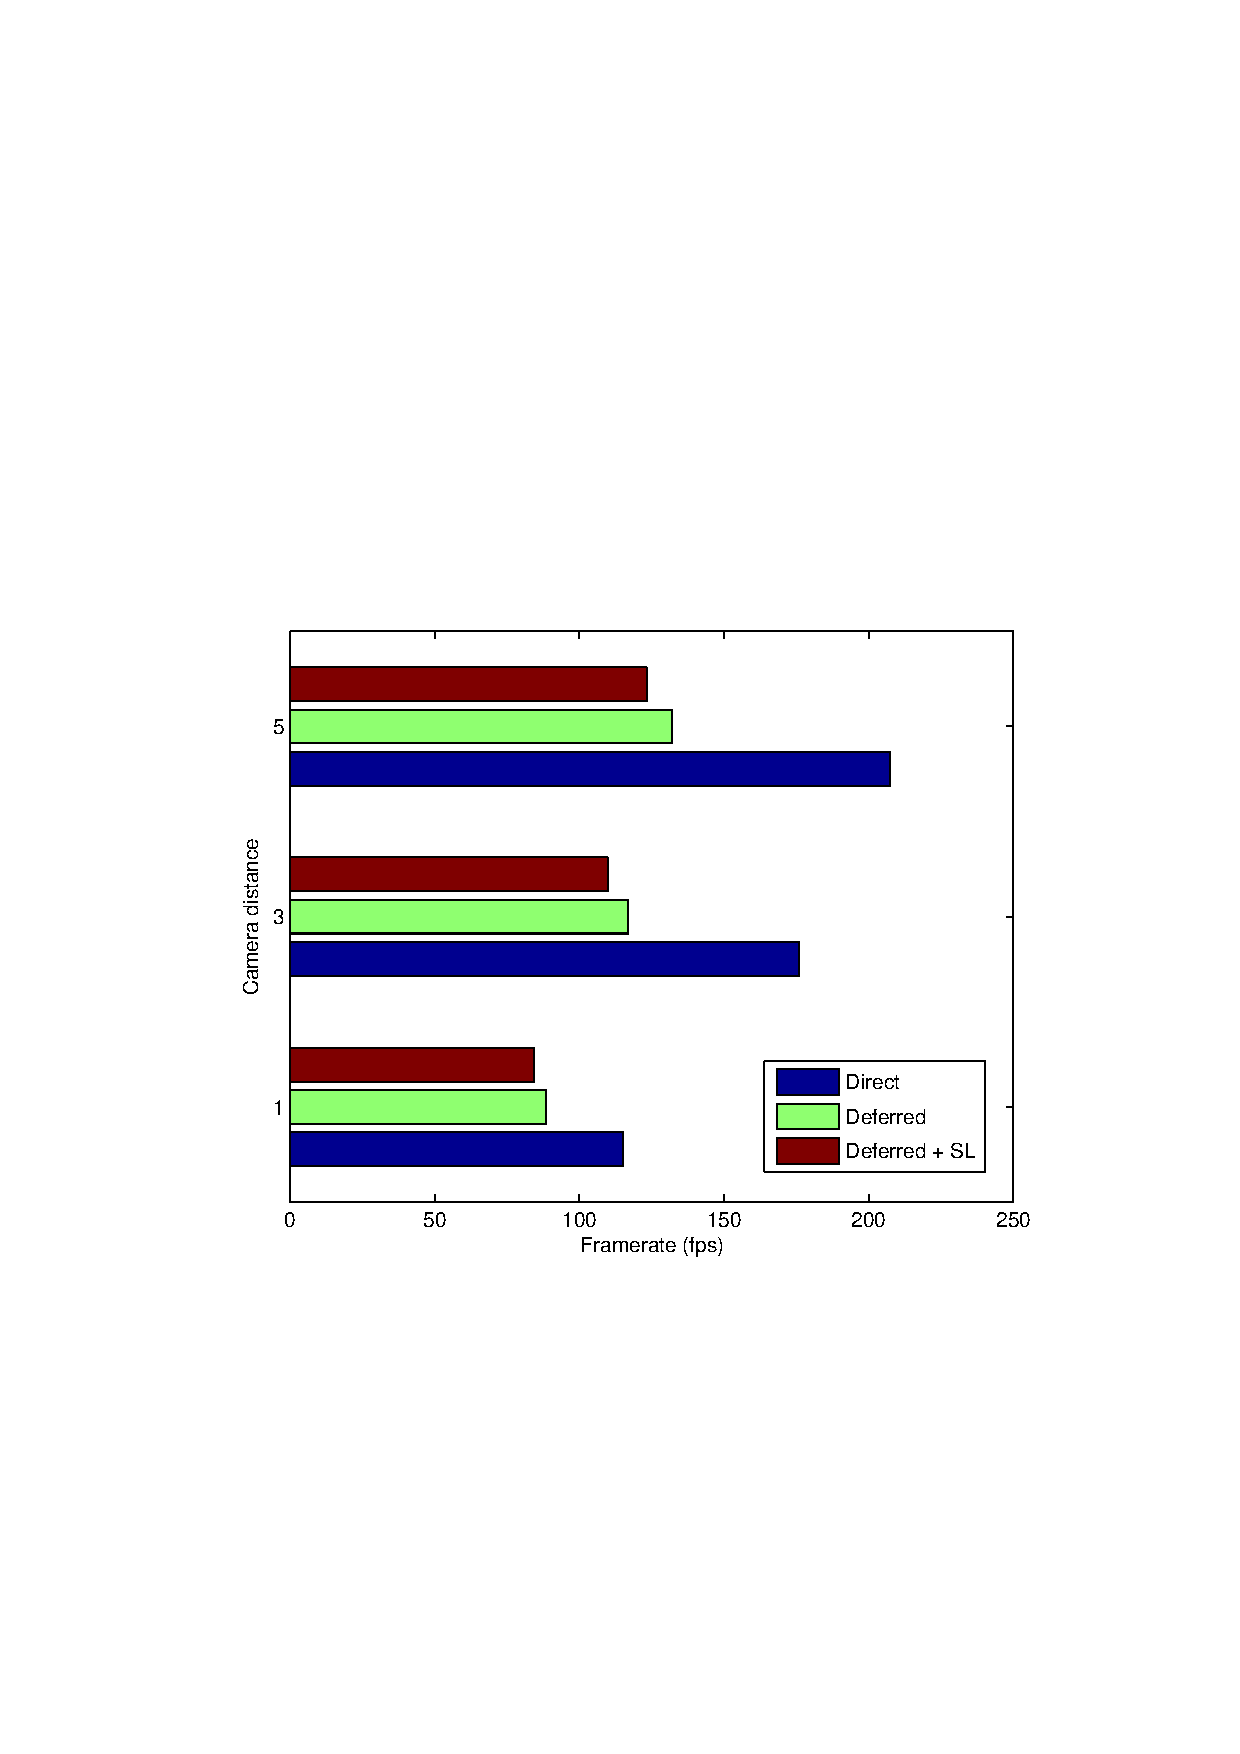
\includegraphics{img/camdist_vs_fps_8600gt_1vqm-lic.pdf}}}
\caption{\em Framerates at different distances of the camera}
\label{f:cam-dist}
\end{figure}

Clearly, having the camera closer to the spheres dramatically decreases performance.
This indicates that the sphere count is not the main factor in determining the rendering speed.
Rather, the number of fragments covered by each sphere, as well as the number of discarded (i.e. wasted) fragments affects performance far stronger.

Also, with data set M at a distance of 1 unit (many large spheres fill up the entire screen), 
deferred shading manages to overtake direct shading in performance.
This suggests that indeed deferred shading can be faster when its memory bandwidth requirements are outweighed by the workload of the shaders.
Nevertheless, deferred shading is only faster when framerates are very low, and then the performance advantage is small.

\subsubsection*{Graphics card comparison}

Finally, we have tested rendering performance among a selection of graphics cards.
This was done using the large and heavy data set N, with the camera distance set to 5 units.
The test results are shown in Figure \ref{f:graka}.

\begin{figure}[!ht]
\centering
\resizebox{100mm}{!}{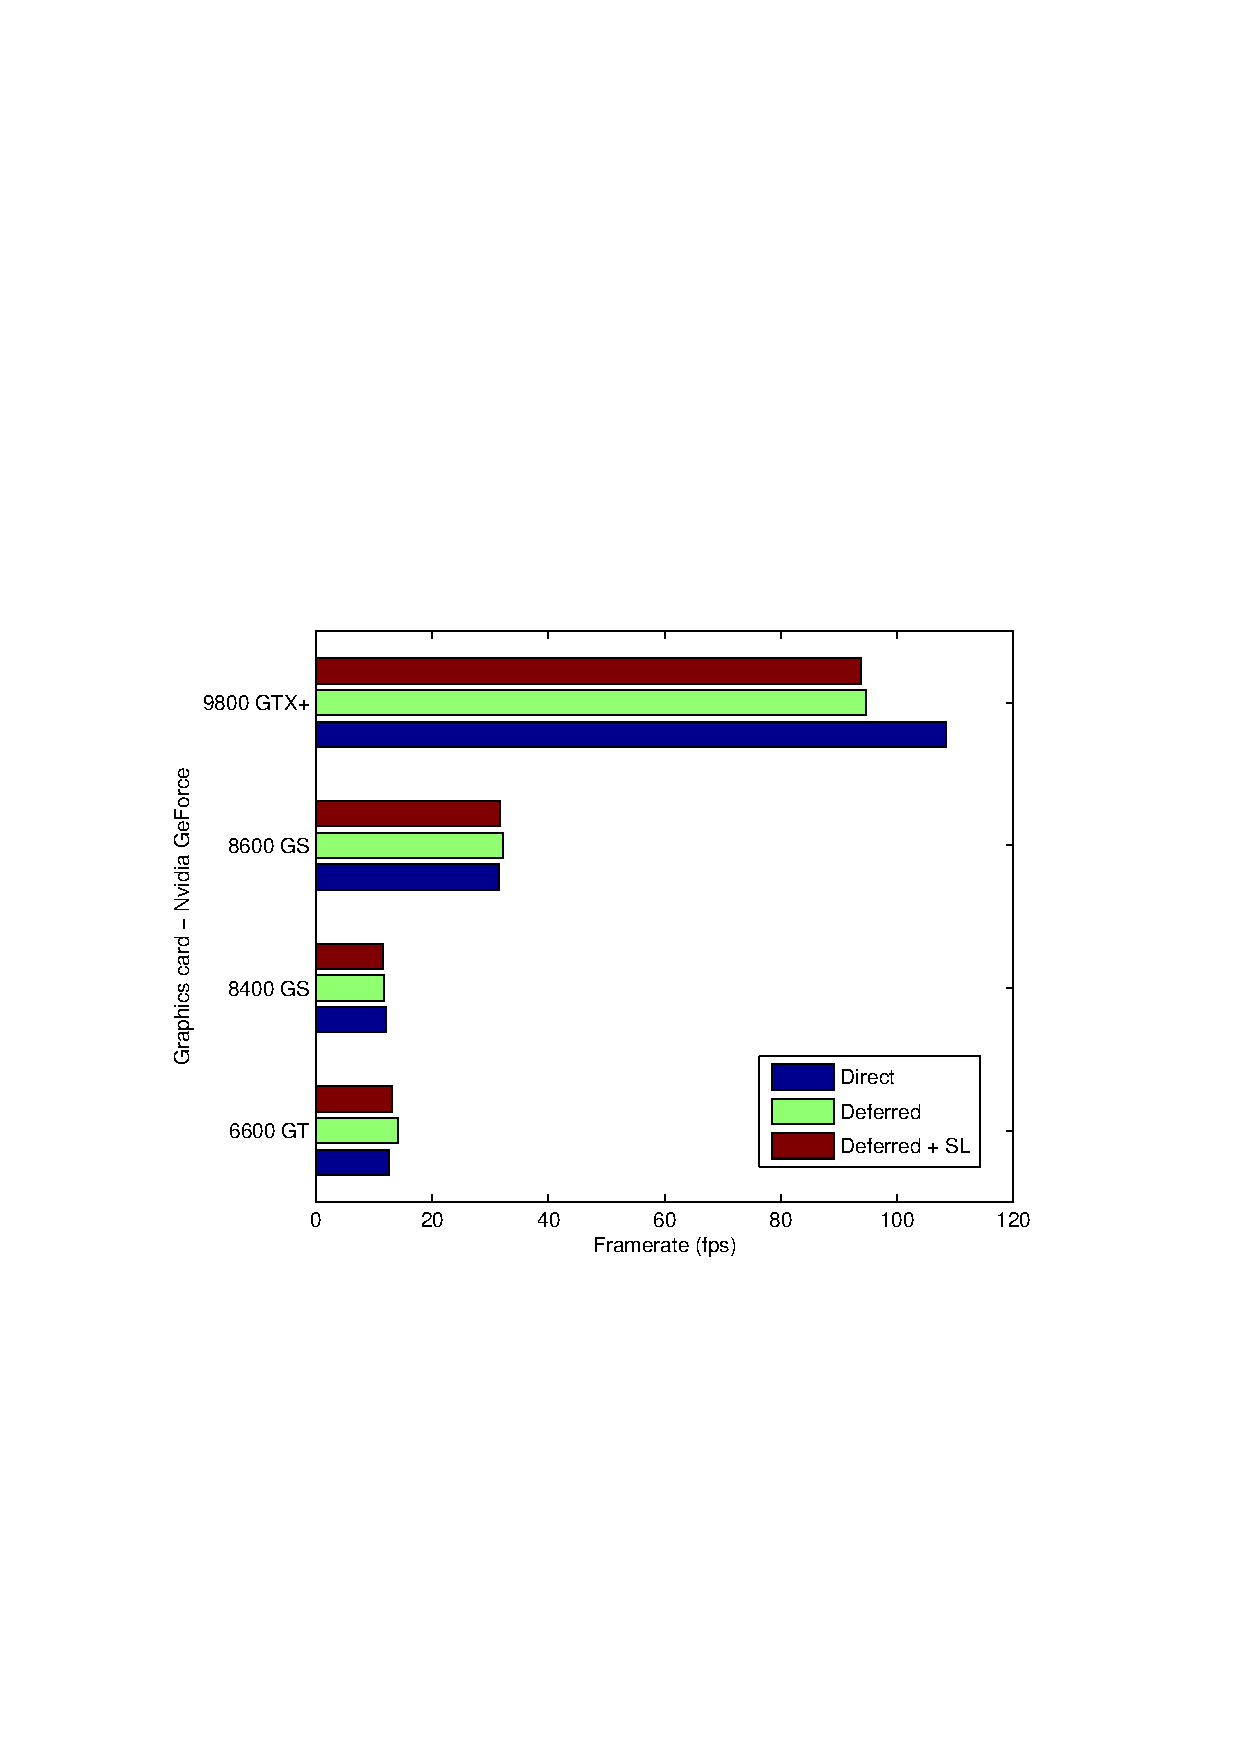
\includegraphics{img/card_vs_fps_1vqm-vdw_cam5.pdf}}
\caption{\em Performance among different graphics cards}
\label{f:graka}
\end{figure}

There is a clear performance improvement from one generation of graphics card to the next, 
so the ray-casting method scales well on faster hardware.
Direct shading is still the winner on the GeForce 9800 GTX+, while deferred shading is a much closer match on the other cards.

\subsection*{Perspective correctness}

According to Sigg's paper, both the bounding box computation and the ray casting methods should produce perspective correct results.
We have tested this by rendering a set of spheres using an extreme perspective (field of vision set to $120\,^{\circ}$), as shown in Figure \ref{f:perspective}.
It is clearly visible that the spheres farthest from the image center are strongly deformed by this perspective and that each sphere's bounding box has been
properly scaled to deal with this deformation (i.e. none of the spheres are cropped). This confirms Sigg's claims.

\begin{figure}[!ht]
\centering
\resizebox{50mm}{!}{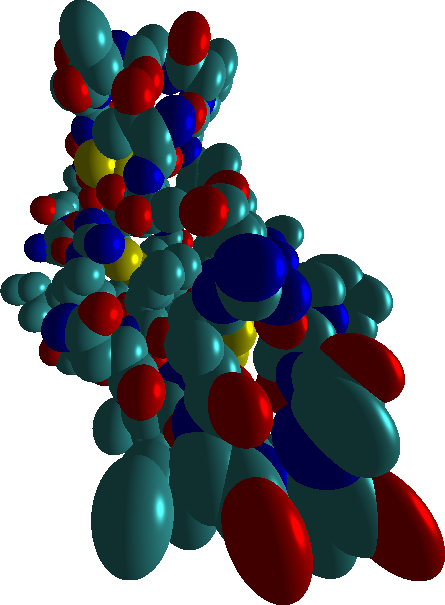
\includegraphics{img/perspective.png}}
\caption{\em Spheres deformed by extreme perspective}
\label{f:perspective}
\end{figure}

\subsection*{Depth perception}

The main reason Sigg added shadow maps to his quadric rendering method was to increase depth perception.
We can not verify this with our own implementation, but it is clear from Sigg's screenshots that self-shadowing greatly improves the ability to see the structure of a model.

Our own implementation shows that indeed the depth perception on still images with only Phong shading is not outstanding.
However, Sigg failed to mention that seeing a model in motion also allows one to get a better grasp on its internal structure, 
which is confirmed by our own observations.
